\chapter{Ubicación de las piezas (placement)}\label{cap:placement}

El \emph{placement} es decidir dónde va cada pieza en la placa. Parece un paso previo sin importancia, pero es al
revés: una vez fijadas las piezas, el ruteo casi se decide solo. Si dos piezas que deben estar unidas quedan lejos,
o si una red queda encerrada por otras, no hay forma de rutear limpio. En este proyecto varios problemas de ruteo se
resolvieron moviendo piezas, no dibujando pistas raras.

En este capítulo vas a ver:
\begin{itemize}
  \item los criterios generales para ubicar piezas, explicados uno por uno;
  \item el mapa final de la placa y por qué cada bloque quedó donde quedó;
  \item la regla de autorización: qué se podía mover sin preguntar y qué necesitaba aprobación;
  \item todos los cambios de placement aprobados, con su motivo;
  \item cómo se usó Freerouting como ``oráculo'' para saber si había camino antes de rutear;
  \item cómo se decidió qué designadores caben en la serigrafía.
\end{itemize}

Las fuentes son \archivo{PLAN_RUTEO.md} (secciones 4, 6, 9, 10, 11.1 y 12), \archivo{REGLAS.md} §3 y §4, y los
archivos de colocación \archivo{tools/ruteo/colocar_bloque*.json} y \archivo{tools/ruteo/alineacion_bloque*.json}.

% =====================================================================================================
\section{Criterios generales de colocación}\label{sec:c07-criterios}

\subsection{1. Agrupar por bloque funcional}
Las piezas de un mismo circuito van juntas: el buck de \SI{3.3}{\volt} con su bobina y sus condensadores, cada
fuente IEPE con sus resistencias, cada AFE con su DAC. Así las conexiones dentro del bloque son cortas, y entre
bloques solo viajan unas pocas redes (la alimentación, la señal de salida). Además, si algo falla en el banco, sabes
en qué rincón de la placa buscar.

\subsection{2. El desacoplo pegado al pin}
Un condensador de desacoplo es un pequeño ``tanque'' de carga junto al integrado. Cuando el integrado pide un pulso
de corriente rápido, lo toma de ahí y no de la fuente, que está lejos. Pero ese pulso tiene que recorrer un lazo:
pin de alimentación $\to$ condensador $\to$ tierra $\to$ pin de tierra. Cuanto más grande el lazo, más inductancia
tiene, y la inductancia se opone justo a los cambios rápidos de corriente. Por eso:
\begin{itemize}
  \item el condensador va lo más cerca posible del pin, con una vía de tierra junto a su pad
        \doc{ADI MT-101};
  \item si hay dos condensadores en paralelo (por ejemplo \SI{100}{\nano\farad} y \SI{10}{\micro\farad}), el
        \emph{pequeño} va más cerca, porque es el que atiende las frecuencias altas;
  \item cada fabricante da su propia distancia:
  \begin{itemize}
    \item el MCP4725 pide el condensador a \SI{4}{\milli\meter} o menos de VDD \doc{DS22039D §8.3};
    \item el PCM1808 pide \SI{0.1}{\micro\farad} + \SI{10}{\micro\farad} ``lo más cerca posible''
          \doc{SLES177B §10.1};
    \item el LMR36015 pide un \SI{220}{\nano\farad} junto a \emph{cada} par VIN/PGND \doc{SNVSB49D §12.1}.
  \end{itemize}
\end{itemize}

\subsection{3. Analógico y digital en zonas, sin partir el plano de tierra}
\begin{idea}[zonas sí, cortes no]
Una idea muy repetida es ``separar la tierra analógica de la digital'' cortando el plano en dos. Las notas de TI y
ADI que se usaron dicen otra cosa: \textbf{un solo plano de tierra, sin cortes}, y la separación se hace
\emph{con la ubicación}. Lo analógico se pone y se rutea solo sobre su zona, y lo digital sobre la suya
\doc{TI SLYT499 p.8, SLYT512 pp.5--6}.

¿Por qué no cortar? Porque la corriente de retorno de una señal vuelve por el plano, justo debajo de la pista (esto
se explica a fondo en el capítulo~\ref{cap:capas}). Si la pista pasa por encima de un corte, el retorno tiene que dar
la vuelta, y el lazo que se forma actúa como una antena. Con el plano entero y las zonas bien separadas, las
corrientes digitales simplemente no pasan por debajo de lo analógico.
\end{idea}

Dos detalles más de esas notas:
\begin{itemize}
  \item \textbf{El convertidor va en la frontera.} El ADC (PCM1808) tiene un lado analógico (entradas, referencia) y
        uno digital (reloj, datos). Se pone justo en el límite entre las dos zonas, con sus pines AGND y DGND unidos
        directamente debajo del encapsulado \doc{SLES177B §10.1.2}.
  \item \textbf{La alimentación entra por el lado digital} \doc{SLYT512}, para que sus corrientes no crucen la
        zona analógica.
\end{itemize}

\subsection{4. El oscilador junto a la entrada de reloj del ADC}
El reloj que marca los instantes de muestreo se trata como una señal \emph{analógica}: cualquier ruido en sus
flancos se convierte en error de muestreo (\emph{jitter}). Por eso el oscilador \net{Y1} va pegado al pin SCKI del
PCM1808, y el reloj no se toma del microcontrolador \copia[MT-031].

\subsection{5. Conectores en el borde}
Los conectores tienen que ser accesibles y aguantar esfuerzo mecánico. Las borneras (\net{J5} entrada de
\SI{24}{\volt}, \net{J1} y \net{J7} habilitación de cada fuente IEPE) van en el borde izquierdo. Los BNC de los
micrófonos (\net{J2}, \net{J8}) van en el borde inferior, con el barril metálico fuera de la placa. La NUCLEO
(\net{A1}) va en el borde derecho con el USB hacia arriba.

\subsection{6. Lo ruidoso, lejos de lo sensible}
Los dos bucks (\net{U6}, \net{U7}) conmutan a \SI{1}{\mega\hertz} y son la mayor fuente de ruido. Van en la franja
superior, junto a la entrada de \SI{24}{\volt} y lejos de los AFE. Dentro de cada buck, el lazo de potencia se
arma según la figura 12-2 del datasheet \doc{SNVSB49D}.

\subsection{7. Lo que pide el ensamblaje}
\begin{itemize}
  \item \textbf{Una sola cara.} PCBA \emph{Economic} monta solo en una cara: todas las piezas SMD van arriba.
  \item \textbf{Cuerpos a \SI{2.5}{\milli\meter} del borde} sin rieles, y \textbf{fiduciales} (capítulo~\ref{cap:jlc}).
  \item \textbf{Las piezas THT se sueldan a mano}: las 8 de \archivo{fabricacion/soldar_a_mano.md} (zócalo de la
        NUCLEO, borneras, BNC y los dos puentes JP1/JP2). Conviene que queden accesibles con el cautín.
\end{itemize}

\subsection{8. Canales iguales}
El canal 2 (micrófono SV 12) es una copia del canal 1 (RG-50). Al final del proceso, el AFE de CH2 quedó con
\textbf{exactamente la misma geometría que el de CH1, desplazada \SI{22.5}{\milli\meter}}. Eso no es estética: dos
canales iguales se comportan igual, se rutean igual y, si uno funciona en el banco y el otro no, la diferencia está
en las piezas y no en el dibujo.

% =====================================================================================================
\section{El mapa de la placa}\label{sec:c07-mapa}

La figura~\ref{fig:c07-mapa} muestra el placement final, coloreado por bloque. Las coordenadas son milímetros desde
la esquina inferior izquierda (en KiCad, el origen está arriba a la izquierda y la $y$ crece hacia abajo; aquí se
dibujó como en un plano normal). Las piezas con borde negro grueso son las que se movieron durante el diseño; están
todas en la sección~\ref{sec:c07-cambios}.

\begin{figure}[!htbp]
\centering
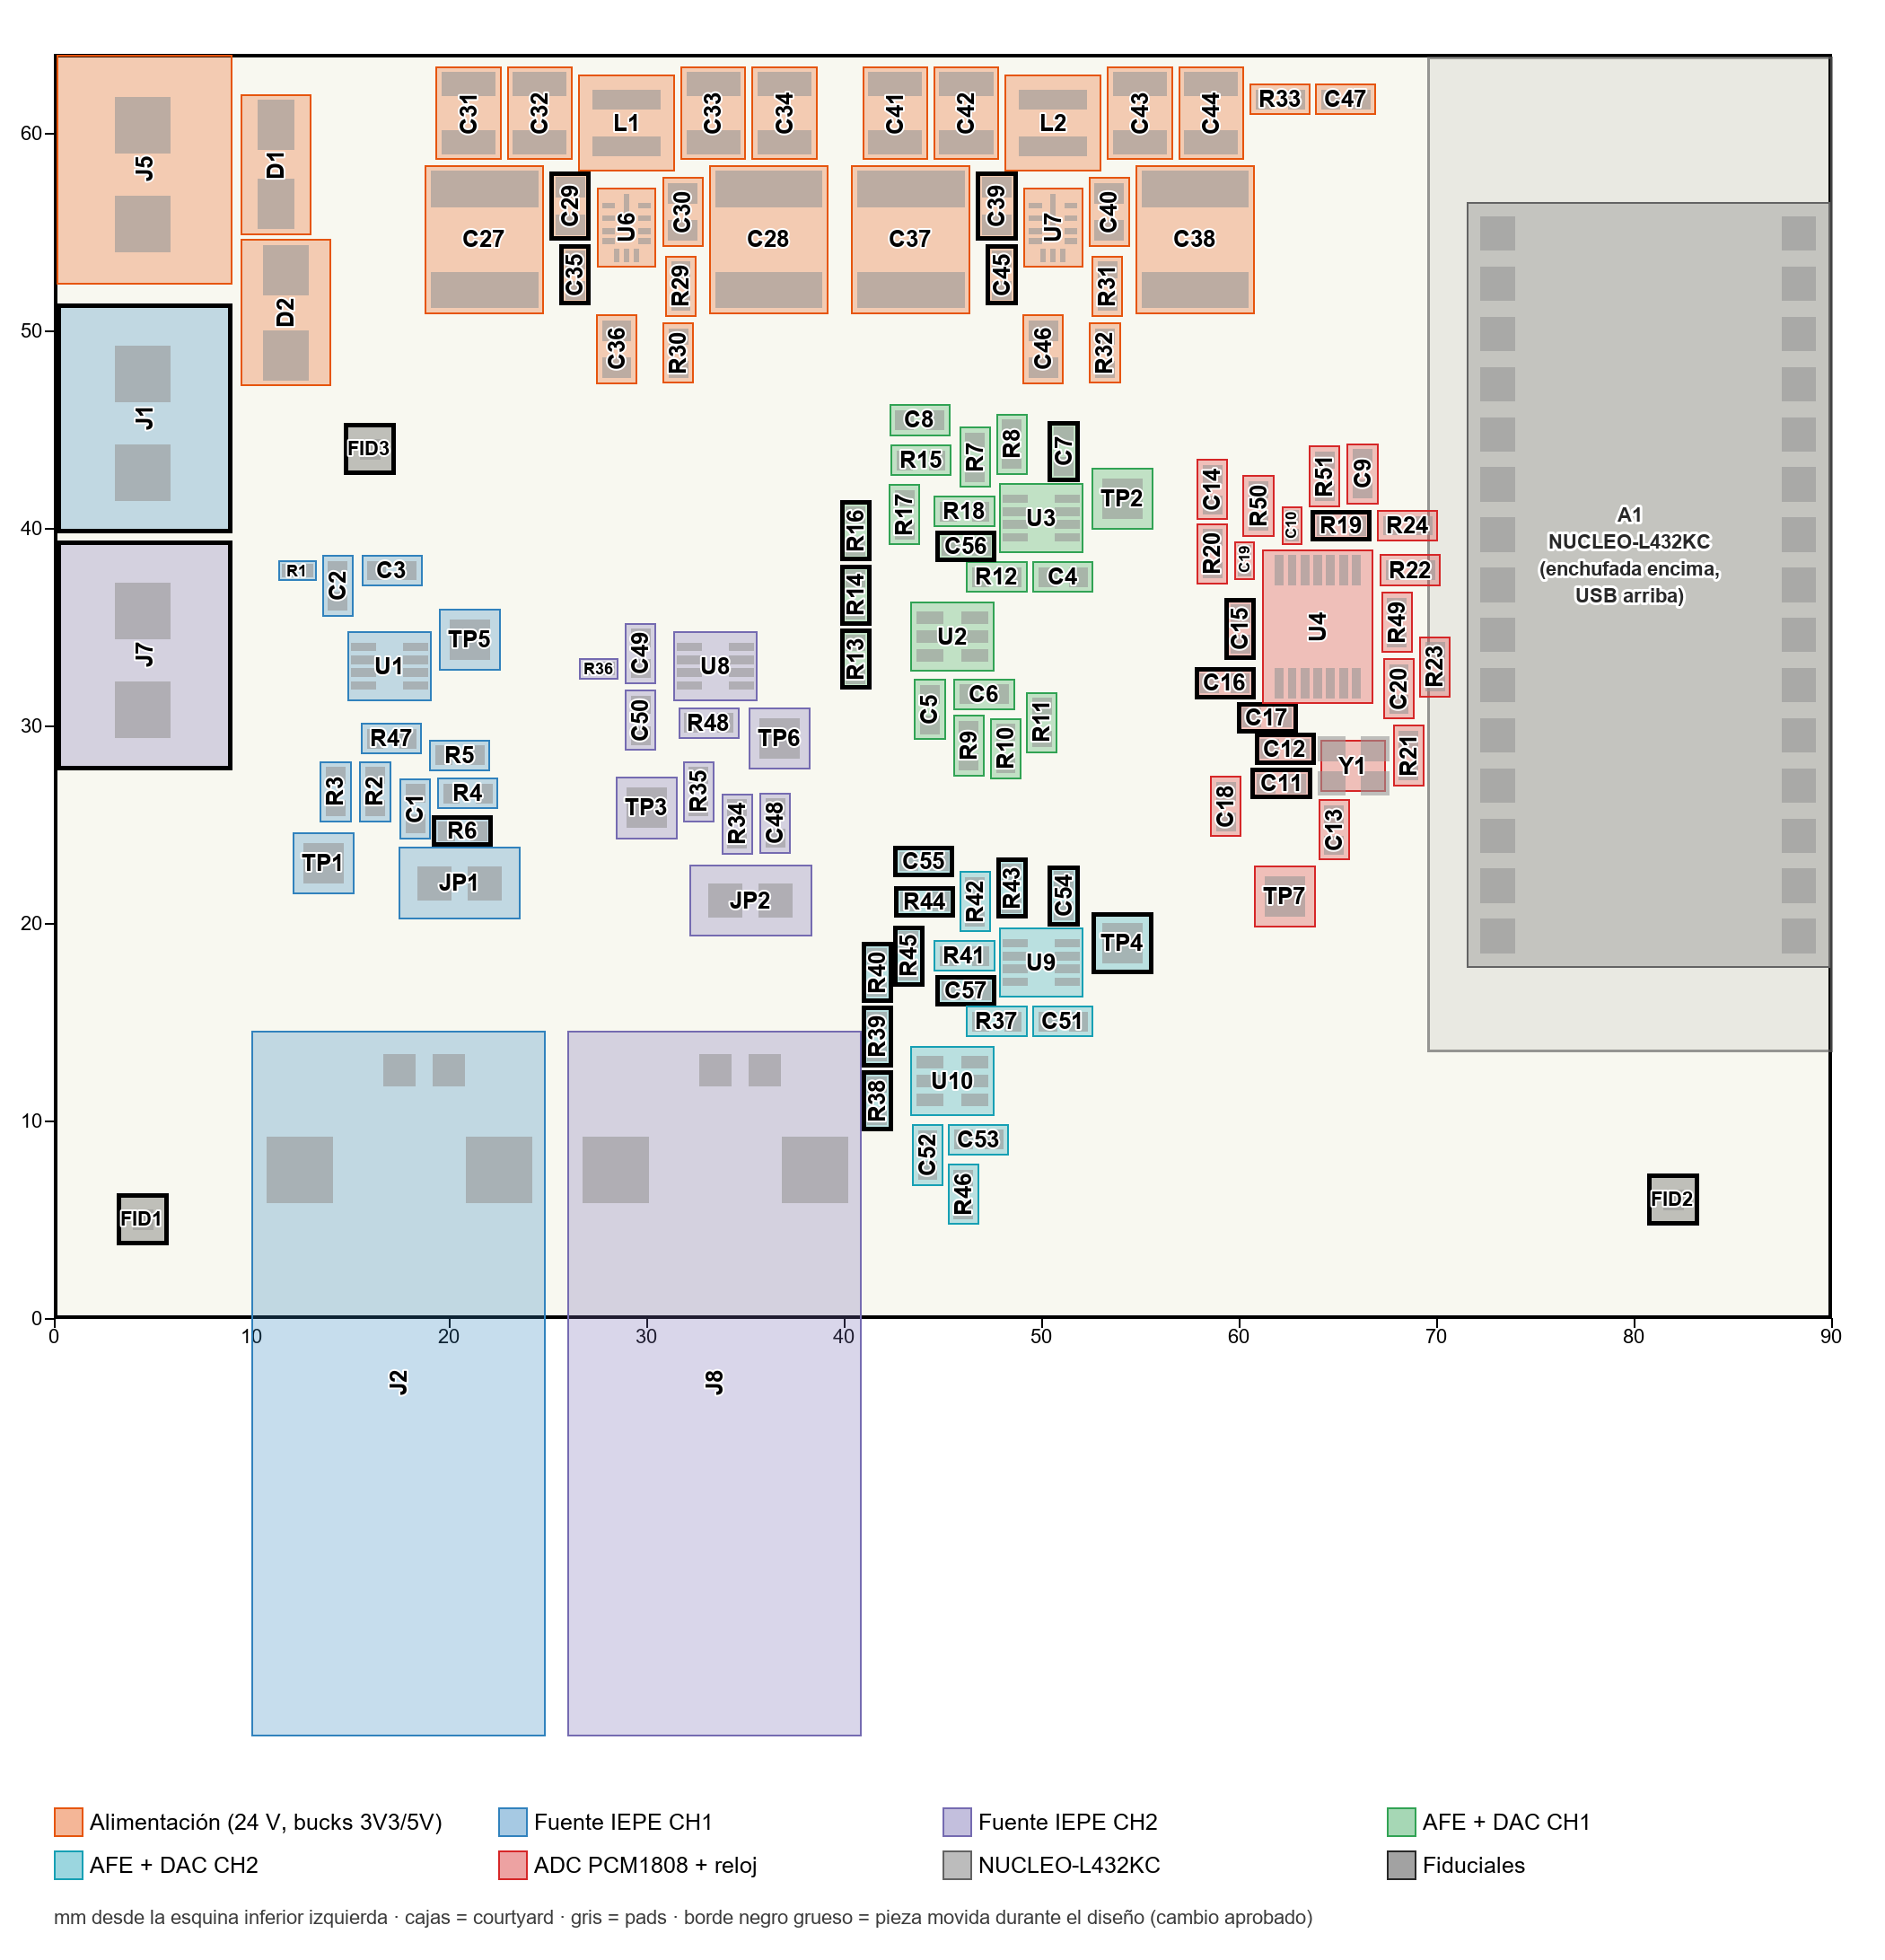
\includegraphics[width=\linewidth]{figuras/c07_mapa_final.png}
\caption{Placement final por bloques, generado a partir de \archivo{pcb.kicad_pcb} (cajas = courtyard, gris =
pads). Los BNC \net{J2} y \net{J8} sobresalen por el borde inferior. Borde negro grueso: pieza movida con un cambio
aprobado.}
\label{fig:c07-mapa}
\end{figure}

Leyendo el mapa de arriba abajo y de izquierda a derecha (posiciones aproximadas, tomadas de la figura):
\begin{itemize}
  \item \textbf{Franja superior, alimentación} ($y \approx 48$ a \SI{64}{\milli\meter}). De izquierda a derecha: la
        bornera de entrada \net{J5}, el diodo serie \net{D1} y el TVS \net{D2}; luego el buck de \SI{3.3}{\volt}
        (\net{U6}, \net{L1}, sus CIN \net{C27}/\net{C28} y sus COUT \net{C31}--\net{C34}) y el de \SI{5}{\volt}
        (\net{U7}, \net{L2}, \net{C37}/\net{C38}, \net{C41}--\net{C44}); al final el filtro \net{R33}/\net{C47} que
        produce \net{5V_A}. Todo lo que conmuta queda en esa franja.
  \item \textbf{Borde izquierdo, conectores}: \net{J5}, \net{J1} y \net{J7}, uno debajo del otro.
  \item \textbf{Centro izquierda, fuentes IEPE}: CH1 (\net{U1} y sus resistencias, $x \approx 12$ a
        \SI{25}{\milli\meter}) y CH2 (\net{U8}, $x \approx 27$ a \SI{40}{\milli\meter}), cada una justo encima de su
        BNC. La corriente sale de la fuente y llega al micrófono por el camino más corto.
  \item \textbf{Centro, los dos AFE}: CH1 arriba ($y \approx 30$ a \SI{47}{\milli\meter}) y CH2 abajo ($y \approx 5$ a
        \SI{25}{\milli\meter}), cada uno con su op-amp (\net{U3}, \net{U9}) y su DAC (\net{U2}, \net{U10}). Las
        columnas de resistencias \net{R13}/\net{R14}/\net{R16} y \net{R38}/\net{R39}/\net{R40} son la cadena de
        \SI{1}{\mega\ohm} de cada canal.
  \item \textbf{Frontera, el ADC} (\net{U4}, $x \approx 58$ a \SI{70}{\milli\meter}): sus entradas miran hacia los AFE
        y su lado digital hacia la NUCLEO. El oscilador \net{Y1} está pegado a él.
  \item \textbf{Borde derecho, zona digital}: la NUCLEO (\net{A1}), de $x \approx 70$ a \SI{90}{\milli\meter}. Por
        debajo de su cuerpo pasan las líneas I2C y DC\_MON hacia sus pines.
\end{itemize}

Para comparar, la figura~\ref{fig:c07-inicial} muestra el placement con el que empezó el ruteo (15 de noviembre).
Ese placement ya estaba verificado (ERC 0, paridad 0, DRC sin errores), pero todavía no tenía ninguna pista: los
problemas solo aparecieron al intentar rutear.

\begin{figure}[!htbp]
\centering
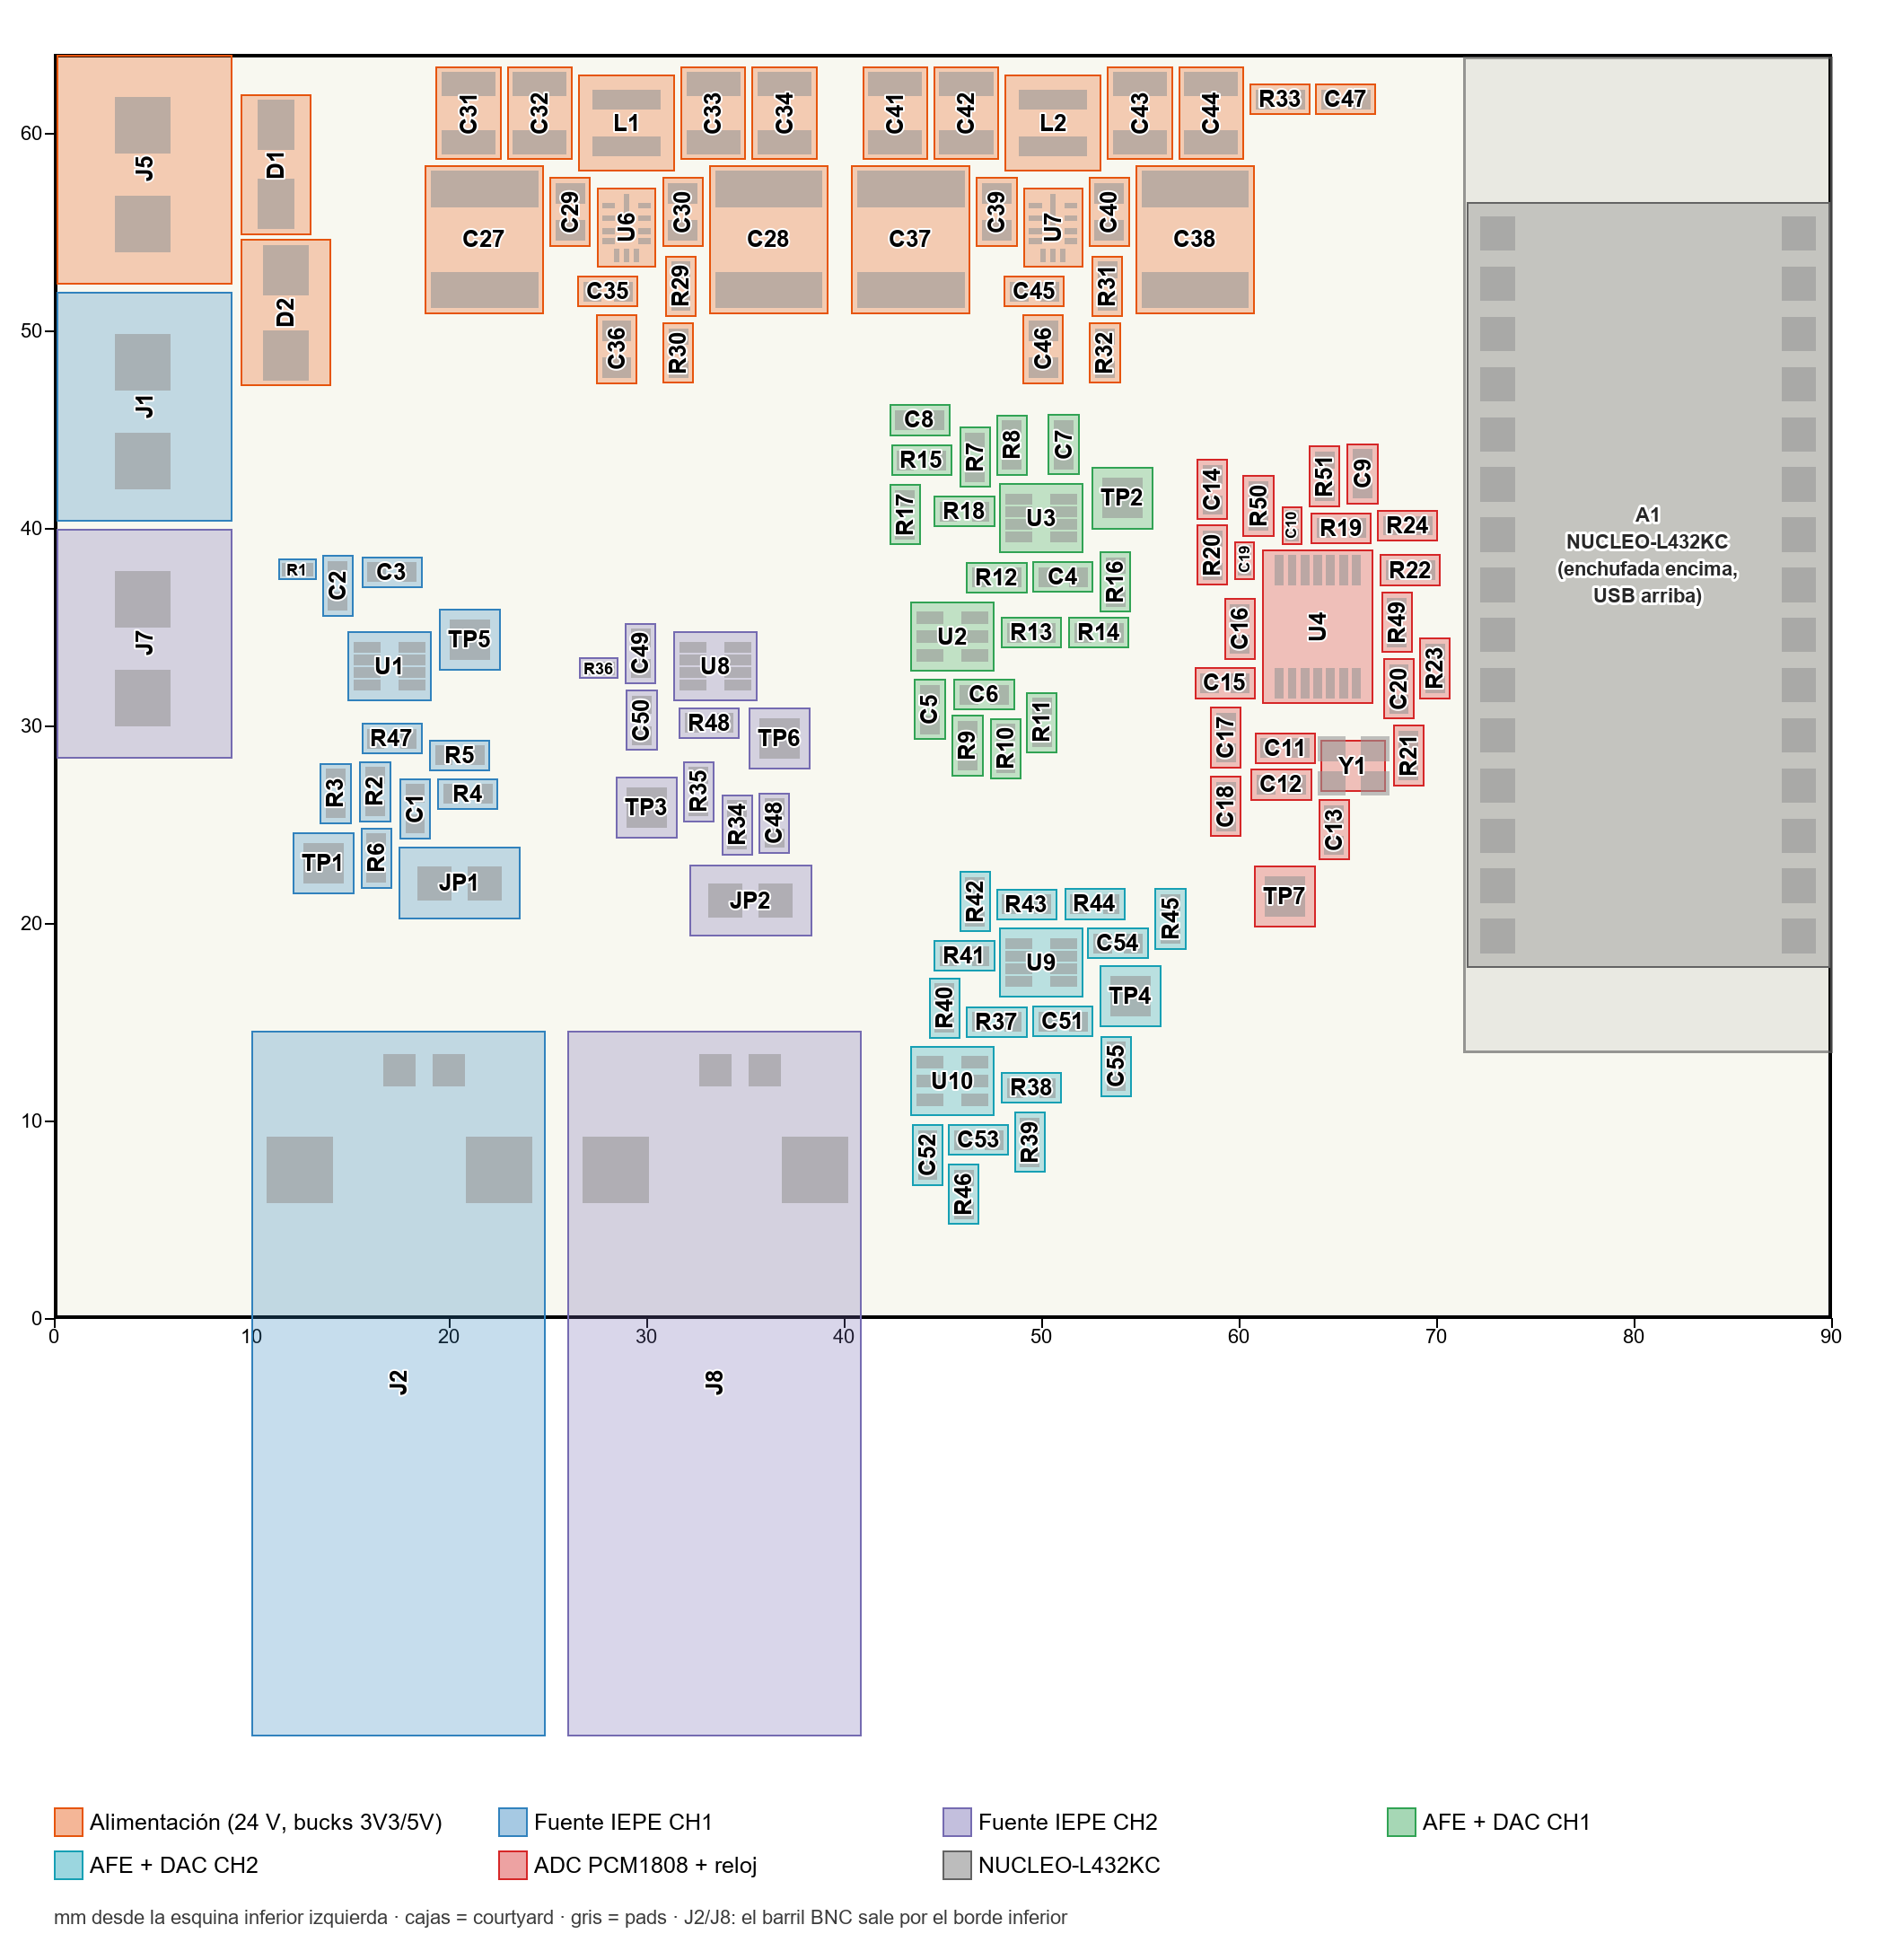
\includegraphics[width=0.66\linewidth]{figuras/placement_map.png}
\caption{Placement inicial de la Rev B, antes de rutear (15/11/2026). Compáralo con la
figura~\ref{fig:c07-mapa}: cambian sobre todo la cadena de \SI{1}{\mega\ohm} de los dos canales, el grupo de
\net{TP4} en CH2 y los desacoplos del ADC.}
\label{fig:c07-inicial}
\end{figure}

% =====================================================================================================
\section{La regla de autorización}\label{sec:c07-autorizacion}

Mover una pieza puede parecer inocente, pero cambia distancias que ya se habían revisado (desacoplos, lazos de
potencia, separaciones). Por eso el dueño del proyecto fijó, el 15/11/2026, dos niveles:

\begin{center}
\begin{tabular}{@{}L{0.46\linewidth}L{0.46\linewidth}@{}}
\toprule
\textbf{Se hace sin preguntar (y se informa al final del bloque)} & \textbf{Se pregunta antes}\\
\midrule
Mover pasivos y puntos de prueba hasta \SI{0.1}{\milli\meter} para alinear pads. &
Mover integrados o conectores.\\
Reubicar textos de serigrafía. & Mover cualquier pieza más de \SI{0.1}{\milli\meter}.\\
Cualquier ajuste que no cambie el esquemático, las piezas ni la topología. &
Cambiar piezas o valores; cualquier excepción a las reglas (DRC, REGLAS.md, chequeo propio).\\
\bottomrule
\end{tabular}
\end{center}

Esta regla está escrita también en el código: la función de alineación de \archivo{tools/eco.py} se niega a mover una
pieza más de \SI{0.1}{\milli\meter} (``supera 0.1 mm (requiere aprobación aparte)''). Los movimientos mayores se
guardan en archivos \archivo{colocar_bloque*.json}, cada uno con el texto de la aprobación, por ejemplo:
\begin{center}
\texttt{"R6": [120.7, 139.35, 180, "aprobado tras el bloque 2: R5.1-R6.1 sin camino\dots"]}
\end{center}

\subsection*{Por qué alinear pads por centésimas de milímetro}
Las reglas de trazado piden quiebres de solo \ang{45}, segmentos de \SI{0.1}{\milli\meter} o más y entrada al pad
por su eje (capítulos~\ref{cap:jlc} y~\ref{cap:ruteo}). Con esas tres reglas, un desfase pequeño entre dos pads
es un problema: si el centro de un pad está \SI{0.05}{\milli\meter} más arriba que el del otro, la pista recta entre
ellos no entra por el eje de ninguno, y para corregirlo harían falta dos quiebres de \ang{45} con un tramo diagonal
de apenas \SI{0.07}{\milli\meter}, más corto que el mínimo (figura~\ref{fig:c07-alinear}). La solución es mover el
pasivo esos \SI{0.05}{\milli\meter} para que los dos pads queden en la misma línea.

\begin{figure}[!htbp]
\centering
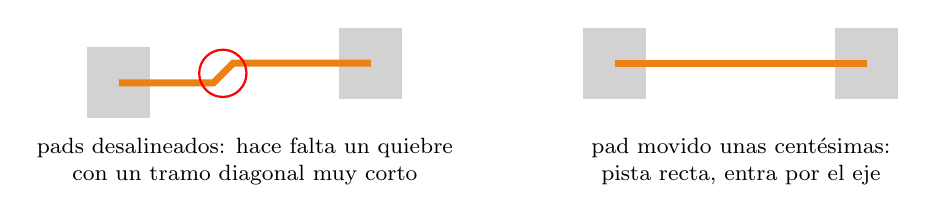
\begin{tikzpicture}[x=1cm,y=1cm,font=\small]
  \begin{scope}
    \fill[gray!35] (0,0) rectangle (0.8,0.9);
    \fill[gray!35] (3.2,0.25) rectangle (4.0,1.15);
    \draw[orange!70!brown,line width=2.5pt] (0.4,0.45) -- (1.6,0.45) -- (1.85,0.7) -- (3.6,0.7);
    \draw[red,thick] (1.72,0.57) circle (0.3);
    \node[align=center,font=\footnotesize] at (2.0,-0.55) {pads desalineados: hace falta un quiebre\\con un tramo diagonal muy corto};
  \end{scope}
  \begin{scope}[xshift=6.3cm]
    \fill[gray!35] (0,0.25) rectangle (0.8,1.15);
    \fill[gray!35] (3.2,0.25) rectangle (4.0,1.15);
    \draw[orange!70!brown,line width=2.5pt] (0.4,0.7) -- (3.6,0.7);
    \node[align=center,font=\footnotesize] at (2.0,-0.55) {pad movido unas centésimas:\\pista recta, entra por el eje};
  \end{scope}
\end{tikzpicture}
\caption{Por qué se alinean los pads (dibujo exagerado; el desfase real era de centésimas de milímetro).}
\label{fig:c07-alinear}
\end{figure}

% =====================================================================================================
\section{Los cambios de placement, uno por uno}\label{sec:c07-cambios}

La tabla~\ref{tab:c07-cambios} lista todos los cambios. Después se explican los que tienen más historia.

{\small
\begin{longtable}{@{}L{0.2\linewidth}L{0.3\linewidth}L{0.3\linewidth}L{0.13\linewidth}@{}}
\caption{Cambios de placement aprobados (PLAN\_RUTEO.md y archivos \archivo{colocar_*}/\archivo{alineacion_*}).}
\label{tab:c07-cambios}\\
\toprule
\textbf{Piezas} & \textbf{Cambio} & \textbf{Por qué} & \textbf{Cuándo}\\
\midrule\endfirsthead
\toprule
\textbf{Piezas} & \textbf{Cambio} & \textbf{Por qué} & \textbf{Cuándo}\\
\midrule\endhead
\net{C29}, \net{C39} (CHF) & suben \SI{0.3}{\milli\meter} & lazo VIN--CHF--PGND más corto & punto de control 2\\
\net{C35}, \net{C45} (CBOOT) & a la izquierda del integrado, girados \ang{90} & camino BOOT--SW corto & punto de control 2\\
\net{C56}, \net{C57} & piezas nuevas, junto a \net{U3} y \net{U9} & condensador CF del sumador (capítulo~\ref{cap:analog}) & punto de control 2\\
\net{J1}, \net{J7} & bajan \SI{0.6}{\milli\meter} & que el designador de \net{J5} quepa sin ambigüedad & punto de control 2\\
\net{FID1}--\net{FID3} & fiduciales nuevos & ensamblaje en JLC & punto de control 2\\
32 pasivos y TP & alineación de $\leq$ \SI{0.094}{\milli\meter} & entrada por el eje del pad & bloque 3\\
\net{R6} & a $(\num{120.70}, \num{139.35})$, horizontal, girado \ang{180} & \net{R5.1}--\net{R6.1} sin camino en una capa & bloque 3\\
\net{R13}, \net{R14}, \net{R16} & columna vertical en $x = \num{140.6}$ & la cadena de \SI{1}{\mega\ohm} de CH1 no tenía camino & análisis de los bloques 4--8\\
\net{R19} & sube \SI{0.1}{\milli\meter} & DOUT a $\geq$ \SI{0.5}{\milli\meter} de las entradas analógicas & bloque 4\\
\net{C17}; \net{C11}$\leftrightarrow$\net{C12}; \net{C15}$\leftrightarrow$\net{C16} & \net{C17} junto a \net{U4.3}; los \SI{100}{\nano\farad} pasan al lugar más cercano al pin & desacoplo del PCM1808 & bloque 4\\
\net{C56}; \net{C4}, \net{C6}, \net{R9} & \SI{+0.08}{\milli\meter}; menos de \SI{1}{\micro\meter} & alineación de pads & bloque 5\\
\net{R38}, \net{R39}, \net{R40} & columna en $x = \num{141.7}$ & el nodo R39--R40 encerraba a \net{U10} & bloque 5\\
\net{C57}, \net{R43} & a las posiciones de \net{C56} y \net{R8} de CH1 & SUM, REST\_SV y el nodo R42--R43 se cruzaban & bloque 5\\
\net{TP4}, \net{C54}, \net{R44}, \net{R45}, \net{C55} & a las posiciones de \net{TP2}, \net{C7}, \net{R15}, \net{R17}, \net{C8} de CH1 & \net{REST_SV} quedaba partido & bloque 5\\
\net{C7} & \SI{0.35}{\milli\meter} más abajo & paso para \net{REST_OUT} sin cortar el desacoplo & bloque 5\\
\bottomrule
\end{longtable}
}

Las coordenadas de esta sección son las de KiCad (milímetros, origen arriba a la izquierda, $y$ hacia abajo),
porque así están en los archivos de colocación.

\subsection{Cambios del punto de control 2}
Antes de trazar la primera pista hubo una revisión general (el ``punto de control 2''). Ahí se aprobaron:
\begin{itemize}
  \item \textbf{Bucks.} Los condensadores de \SI{220}{\nano\farad} entre VIN y PGND (\net{C29}, \net{C39}) subieron
        \SI{0.3}{\milli\meter}, y los de BOOT (\net{C35}, \net{C45}) pasaron a la izquierda del integrado, girados
        \ang{90}. El objetivo era el que pide TI: el lazo VIN--CHF--PGND lo más pequeño posible y el condensador de
        BOOT cerca de BOOT y SW \doc{SNVSB49D §12.1}. En el capítulo~\ref{cap:ruteo} están las medidas de esos lazos.
  \item \textbf{CF.} Los condensadores nuevos \net{C56} y \net{C57} se pusieron entre los pines 1 y 2 de cada op-amp,
        que es justo donde se conectan (salida y entrada inversora del sumador).
  \item \textbf{J1 y J7 bajan \SI{0.6}{\milli\meter}.} El designador de \net{J5} es obligatorio (los conectores nunca
        se omiten de la serigrafía) y con las borneras pegadas no había forma de ponerlo sin que se confundiera con
        el de \net{J1}. Se probó en una copia: el DRC no mostró errores nuevos. En la placa, \net{J1} pasó de
        $y = \num{115.6}$ a \num{116.2} y \net{J7} de \num{127.6} a \num{128.2} \medido. Son borneras soldadas a mano.
  \item \textbf{Fiduciales} \net{FID1}--\net{FID3} en $(\num{4.5}, \num{5})$, $(\num{82}, \num{6})$ y
        $(\num{16}, \num{44})$~\si{\milli\meter} desde la esquina inferior izquierda, a \SI{6}{\milli\meter} o más del
        pad más cercano.
\end{itemize}

\subsection{R6: sin camino en una capa}
En el bloque 3 (fuentes IEPE), el enlace \net{R5.1}--\net{R6.1} no tenía camino en una sola capa con \net{R6} en su
lugar original $(\num{116.27}, \num{140.72})$: Freerouting lo dejó sin rutear después de 800 pasadas. Con \net{R6} en
$(\num{120.70}, \num{139.35})$, horizontal y girado \ang{180}, el enlace sale completo. Es una resistencia, pero el
movimiento es de más de \SI{4}{\milli\meter}, así que se pidió aprobación.

\subsection{La columna de la cadena de \SI{1}{\mega\ohm}}
La entrada de cada AFE es una cadena de cuatro resistencias en serie que suma \SI{1}{\mega\ohm}
(\SI{390}{\kilo\ohm} + \SI{365}{\kilo\ohm} + \SI{191}{\kilo\ohm} + \SI{54.9}{\kilo\ohm}). Es un nodo de \emph{alta
impedancia}: cualquier pista que pase cerca le acopla ruido, así que no se le pueden pasar puentes por debajo ni
cruzarlo.

En CH1 había un problema. \net{R14} y \net{R16} estaban a la derecha de \net{U3}, y \net{U3} quedaba ``cerrado'' por
sus propias redes (\net{REST_OUT} hacia \net{R8}, \net{5V_A} hacia \net{C7}, la entrada del seguidor hacia
\net{C4}/\net{R12}, y SUM). El oráculo (sección~\ref{sec:c07-oraculo}) dejaba sin rutear dos enlaces: IEPE hasta
\net{R13.2} y el final de la cadena, \net{R16} hasta \net{R18}.

\begin{decision}[R13, R14 y R16 en columna]
\textbf{Qué se decidió:} poner \net{R13}, \net{R14} y \net{R16} verticales y apiladas en la columna libre
$x = \num{140.6}$ (commit \texttt{0452393}, \archivo{colocar_bloque5.json}).

\textbf{Alternativas:} pasar la cadena por debajo de otras piezas o en otra capa. Ninguna sirve: es un nodo de alta
impedancia.

\textbf{Por qué:} con la columna, IEPE entra a \net{R13} por la izquierda sin meterse al AFE, y la cadena sube y
entra a \net{R18.2} pasando entre los pads de \net{R17}. En la prueba del oráculo, \textbf{todas las redes críticas
de los bloques 4 a 7 salieron en \capa{F.Cu} con 0 vías} (figura~\ref{fig:c07-oraculo}). El DRC no mostró solapes
de courtyard.

\textbf{Fuente:} \archivo{PLAN_RUTEO.md} §10 y §10.1.
\end{decision}

\begin{figure}[!htbp]
\centering
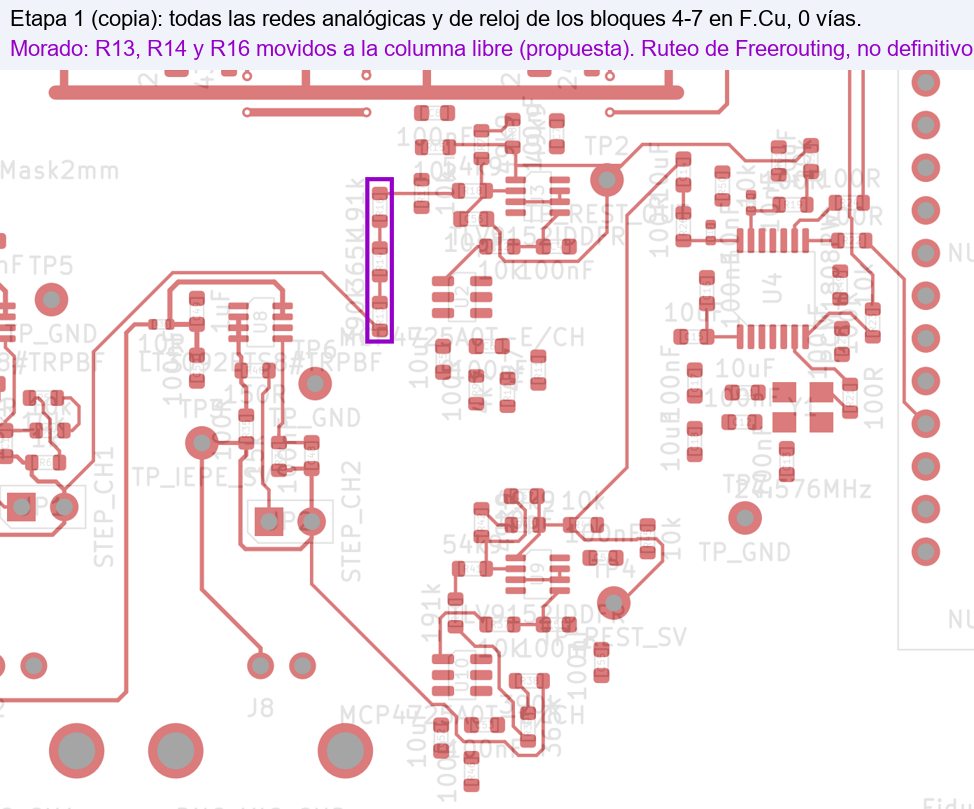
\includegraphics[width=0.78\linewidth]{figuras/oraculo_etapa1_columna.png}
\caption{Prueba del oráculo (en una copia, no es el ruteo final): las redes analógicas y de reloj de los bloques
4--7 en \capa{F.Cu}, sin vías. En morado, \net{R13}, \net{R14} y \net{R16} en la columna libre.}
\label{fig:c07-oraculo}
\end{figure}

\subsection{Los desacoplos del ADC}
Después del bloque 4, el chequeo de desacoplo encontró varios condensadores del PCM1808 lejos de sus pines. Se
aprobó (\archivo{colocar_bloque4.json}):
\begin{itemize}
  \item \net{C17} (\SI{100}{\nano\farad} de \net{5V_A}) junto al pin 3 de \net{U4}, a \SI{0.71}{\milli\meter};
  \item intercambiar \net{C11}$\leftrightarrow$\net{C12} y \net{C15}$\leftrightarrow$\net{C16}, para que el de
        \SI{100}{\nano\farad} quede en el lugar más cercano al pin y el de \SI{10}{\micro\farad} un poco más lejos.
\end{itemize}
Es el criterio 2 de arriba: el condensador pequeño atiende las frecuencias altas y su lazo debe ser el más corto. Aun
así, \net{C12} (\SI{2.12}{\milli\meter}) y \net{C16} (\SI{1.32}{\milli\meter}) quedaron por encima del límite de
\SI{1}{\milli\meter} del chequeo y se aceptaron como excepción (capítulo~\ref{cap:banco}).

También en el bloque 4, \net{R19} subió \SI{0.1}{\milli\meter} (un ajuste autorizado) para que la pista de datos
DOUT pase por debajo de ella a \SI{0.5}{\milli\meter} o más de \net{AC_LEFT}/VINL, que es lo que exige la regla
\net{reloj_lejos_de_analogica}.

\subsection{CH2: hacerlo igual a CH1}
Con la colocación original, CH2 no se podía rutear limpio:
\begin{itemize}
  \item el nodo entre \net{R39} y \net{R40} rodeaba a \net{U10} y encerraba sus salidas SCL (\net{U10.5}) y A0
        (\net{U10.6});
  \item en el grupo de \net{C57}/\net{R43}, las redes SUM, \net{REST_SV} y el nodo R42--R43 se cruzaban: hacían
        falta tres entradas a pads en diagonal, contra la regla de entrar por el eje.
\end{itemize}
Primero se probó la solución en una copia y luego se aprobó en dos pasos:
\begin{enumerate}
  \item \archivo{colocar_bloque5b.json}: \net{R38}, \net{R39} y \net{R40} en columna en $x = \num{141.7}$ (el courtyard
        de \net{J8} llega hasta $x = \num{140.90}$, por eso no se pudo usar $\num{140.6}$ como en CH1); \net{C57} en
        el lugar equivalente al de \net{C56}, $(\num{146.19}, \num{147.43})$; y \net{R43} vertical como \net{R8}.
  \item \archivo{colocar_bloque5c.json}: aun así \net{REST_SV} quedaba partido en dos grupos,
        \{\net{U9.1}, \net{R43.1}, \net{R44.2}\} y \{\net{C57.2}, \net{TP4}\}, porque \net{TP4} estaba encerrado por
        \net{DC_MON2}, \net{C54} y la conexión de \net{5V_A} a \net{U9.8}. Se movieron \net{TP4}, \net{C54},
        \net{R44}, \net{R45} y \net{C55} a los lugares equivalentes de \net{TP2}, \net{C7}, \net{R15}, \net{R17} y
        \net{C8} de CH1 (\net{R44}, \net{R45} y \net{C55} van \SI{0.2}{\milli\meter} más a la derecha, por la
        columna).
\end{enumerate}
El resultado: \textbf{CH2 es CH1 desplazado \SI{22.5}{\milli\meter}}. \net{C57}, \net{R41} y \net{R42} perdieron su
designador en la serigrafía (no cabía) y quedan en el PDF de montaje.

\subsection{C7}
\net{REST_OUT} (la salida del sumador de CH1) tiene que salir de \net{U3.1} hacia la derecha. No cabía entre
\net{U3.8} y su condensador de desacoplo \net{C7} sin cortar el desacoplo. Se bajó \net{C7} \SI{0.35}{\milli\meter}
en total (una alineación de \SI{0.1}{\milli\meter} más \SI{0.25}{\milli\meter} aprobados); queda a
\SI{0.975}{\milli\meter} de \net{U3.8}, todavía dentro del límite de \SI{1}{\milli\meter}, y \net{REST_OUT} pasa por
encima de \net{C7} hacia \net{TP2}.

% =====================================================================================================
\section{Freerouting como oráculo}\label{sec:c07-oraculo}

Freerouting es un \emph{autorouter} libre: le das las piezas y las conexiones y busca pistas que las unan. En este
proyecto \textbf{nunca se usó para el ruteo final}, que se hizo a mano con polilíneas (capítulo~\ref{cap:ruteo}). Se
usó como \emph{oráculo}: en una copia de la placa se le pregunta ``¿existe un camino?'', y su respuesta orienta el
placement. Si un autorouter con cientos de pasadas no encuentra camino para un enlace, es una señal fuerte de que
hay que mover algo.

\begin{ojo}[un oráculo también se equivoca]
La primera prueba de factibilidad con Freerouting tuvo varios problemas, documentados en \archivo{PLAN_RUTEO.md}
§1.2: no se guardó el resultado (así que no se sabía qué conexiones fallaban), usaba los pads viejos del TSOT y
pistas anchas en pines de paso fino (parte de las fallas podían ser de acceso a pines y no cruces), y el límite de
pasadas no se aplicó porque la opción tenía otro nombre. Además, dos procesos quedaron vivos y ocuparon unos
\SI{6}{\giga\byte} de memoria. Por eso sus resultados se tomaron como \emph{indicio}, no como prueba, y las corridas
siguientes se hicieron con memoria limitada, límite de pasadas y guardando el resultado.
\end{ojo}

El análisis de los bloques 4 a 8 se hizo en dos etapas (\archivo{tools/ruteo/oraculo/}):
\begin{enumerate}
  \item \textbf{Redes críticas solas} (analógicas y de reloj, solo en \capa{F.Cu}). Con el placement original
        quedaban sin rutear los dos enlaces de la cadena de CH1. Con la columna, todo salió en \capa{F.Cu} con 0
        vías (figura~\ref{fig:c07-oraculo}).
  \item \textbf{El resto} (alimentación, I2C, DC\_MON, straps) con lo crítico congelado. En 2 capas, o se usaban
        unos \SI{140}{\milli\meter} de \capa{B.Cu} pasando bajo unas 12 redes críticas (y quedaban 3 sin rutear), o
        se penalizaban las vías y quedaban 17 sin rutear. Esta etapa fue la que llevó a la placa de 4 capas
        (capítulo~\ref{cap:capas}).
\end{enumerate}

% =====================================================================================================
\section{Serigrafía y el PDF de montaje}\label{sec:c07-serigrafia}

La serigrafía también es parte del placement: cada designador (``R13'', ``C7'') tiene que caber cerca de su pieza
sin tapar nada. Las reglas, aplicadas por \archivo{tools/ruteo/serigrafia.py}, son:
\begin{itemize}
  \item texto de \SI{1.0}{\milli\meter} de alto y \SI{0.15}{\milli\meter} de trazo (mínimo de JLC), solo a \ang{0} o
        \ang{90} (se lee desde abajo o desde la derecha);
  \item nunca sobre pads (con \SI{0.15}{\milli\meter} de separación), vías, máscara abierta ni sobre el cuerpo de
        ninguna pieza; sin solaparse con otra serigrafía; a \SI{0.5}{\milli\meter} o más del borde;
  \item \textbf{sin ambigüedad}: el texto debe quedar más cerca de su pieza que de cualquier otra del mismo tipo;
  \item si no cabe, el designador se omite. \textbf{Nunca} se omiten las marcas de pin 1 y de polaridad, los
        conectores (\net{J*}, \net{A1}, \net{JP*}) ni los puntos de prueba (\net{TP*}).
\end{itemize}

El script prueba posiciones alrededor de cada pieza (a varias distancias y corrimientos) y se queda con la primera que
cumple todo. El número de omitidos fue cambiando: 28 antes de rutear, 18 con el bloque 1 y \textbf{21 al final}:
\begin{center}
\net{C10} \net{C12} \net{C19} \net{C20} \net{C29} \net{C30} \net{C32} \net{C33} \net{C39} \net{C40} \net{C42}
\net{C43} \net{C57} \net{L1} \net{L2} \net{R7} \net{R18} \net{R19} \net{R22} \net{R41} \net{R42}
\end{center}

Para no perderlos, \archivo{fabricacion/montaje.pdf} dibuja la capa \capa{F.Fab} con \emph{todos} los designadores
dentro del cuerpo de cada pieza (es vectorial: con zoom se leen), y \archivo{fabricacion/LEEME.md} trae una tabla con
la posición de cada omitido.

\begin{ojo}[el orden importa]
Las vías de cosido de tierra (capítulo~\ref{cap:ruteo}) también ocupan lugar. Al principio se ponían antes de la
serigrafía, y entonces varios designadores más se quedaban sin lugar. Se invirtió el orden: primero se coloca la
serigrafía y después \archivo{cosido.py} pone las vías evitando toda la serigrafía. Así se volvió a los mismos 21
omitidos. Además, como
las vías van taponadas, el DRC no ve un texto encima de una vía; para eso se agregó el chequeo M a
\archivo{revisar_pistas.py} (capítulo~\ref{cap:verif}).
\end{ojo}

% =====================================================================================================
\section*{Resumen}
\begin{itemize}
  \item El placement sigue ocho criterios: bloques juntos, desacoplo pegado al pin (el pequeño más cerca), zonas
        analógica y digital sin cortar el plano, ADC en la frontera, oscilador junto a SCKI, conectores al borde, lo
        ruidoso lejos de lo sensible y lo que pide el ensamblaje.
  \item La placa quedó en franjas: alimentación arriba, conectores a la izquierda, fuentes IEPE sobre sus BNC, los
        dos AFE en el centro, el ADC en la frontera y la NUCLEO a la derecha.
  \item Mover más de \SI{0.1}{\milli\meter}, o mover integrados y conectores, necesitó aprobación. Cada movimiento
        aprobado está en un archivo \archivo{colocar_bloque*.json} con su motivo.
  \item Los cambios más importantes fueron la columna de la cadena de \SI{1}{\mega\ohm} en los dos canales y dejar CH2
        idéntico a CH1 desplazado \SI{22.5}{\milli\meter}.
  \item Freerouting se usó solo como oráculo de factibilidad en copias; su segunda etapa mostró que en 2 capas no
        había solución limpia.
  \item 21 designadores no caben en la serigrafía; están en \archivo{fabricacion/montaje.pdf}.
\end{itemize}
